% $Id$
\documentclass[11pt]{article}

% DEFAULT PACKAGE SETUP

\usepackage{setspace,graphicx,epstopdf,amsmath,amsfonts,amssymb,amsthm,versionPO}
\usepackage{marginnote,datetime,enumitem,subfigure,rotating,fancyvrb}
\usepackage{hyperref,float}
\usepackage[longnamesfirst]{natbib}
\usdate

% These next lines allow including or excluding different versions of text
% using versionPO.sty

\excludeversion{notes}		% Include notes?
\includeversion{links}          % Turn hyperlinks on?

% Turn off hyperlinking if links is excluded
\iflinks{}{\hypersetup{draft=true}}

% Notes options
\ifnotes{%
\usepackage[margin=1in,paperwidth=10in,right=2.5in]{geometry}%
\usepackage[textwidth=1.4in,shadow,colorinlistoftodos]{todonotes}%
}{%
\usepackage[margin=1in]{geometry}%
\usepackage[disable]{todonotes}%
}

% Allow todonotes inside footnotes without blowing up LaTeX
% Next command works but now notes can overlap. Instead, we'll define 
% a special footnote note command that performs this redefinition.
%\renewcommand{\marginpar}{\marginnote}%

% Save original definition of \marginpar
\let\oldmarginpar\marginpar

% Workaround for todonotes problem with natbib (To Do list title comes out wrong)
\makeatletter\let\chapter\@undefined\makeatother % Undefine \chapter for todonotes

% Define note commands
\newcommand{\smalltodo}[2][] {\todo[caption={#2}, size=\scriptsize, fancyline, #1] {\begin{spacing}{.5}#2\end{spacing}}}
\newcommand{\rhs}[2][]{\smalltodo[color=green!30,#1]{{\bf RS:} #2}}
\newcommand{\rhsnolist}[2][]{\smalltodo[nolist,color=green!30,#1]{{\bf RS:} #2}}
\newcommand{\rhsfn}[2][]{%  To be used in footnotes (and in floats)
\renewcommand{\marginpar}{\marginnote}%
\smalltodo[color=green!30,#1]{{\bf RS:} #2}%
\renewcommand{\marginpar}{\oldmarginpar}}
%\newcommand{\textnote}[1]{\ifnotes{{\noindent\color{red}#1}}{}}
\newcommand{\textnote}[1]{\ifnotes{{\colorbox{yellow}{{\color{red}#1}}}}{}}

% Command to start a new page, starting on odd-numbered page if twoside option 
% is selected above
\newcommand{\clearRHS}{\clearpage\thispagestyle{empty}\cleardoublepage\thispagestyle{plain}}

% Number paragraphs and subparagraphs and include them in TOC
\setcounter{tocdepth}{2}

% JF-specific includes:

\usepackage{indentfirst} % Indent first sentence of a new section.
\usepackage{endnotes}    % Use endnotes instead of footnotes
\usepackage{jf}          % JF-specific formatting of sections, etc.
\usepackage[labelfont=bf,labelsep=period, font=small]{caption}   % Format figure captions
\captionsetup[table]{labelsep=none}

% Define theorem-like commands and a few random function names.
\newtheorem{condition}{CONDITION}
\newtheorem{corollary}{COROLLARY}
\newtheorem{proposition}{PROPOSITION}
\newtheorem{obs}{OBSERVATION}
\newcommand{\argmax}{\mathop{\rm arg\,max}}
\newcommand{\sign}{\mathop{\rm sign}}
\newcommand{\defeq}{\stackrel{\rm def}{=}}

\title{\Large \bf Literature Review on Money Market Mutual Funds}
\author{ADARSH KUTHURU}
\date{\parbox{\linewidth}{\centering%
  \today\endgraf\bigskip
  \endgraf\medskip
  PhD Student in Finance \endgraf
  Boston College, United States}}
  
\begin{document}

\maketitle
\thispagestyle{empty}
\bigskip
\clearpage
\tableofcontents

\setlist{noitemsep}  % Reduce space between list items (itemize, enumerate, etc.)
\onehalfspacing      % Use 1.5 spacing
% Use endnotes instead of footnotes - redefine \footnote command
\renewcommand{\footnote}{\endnote}  % Endnotes instead of footnotes

\clearpage


% Create title page with no page number


\section{Introduction} \label{sec:Intro}

In this literature review on money market mutual funds (MMMF), I focus mainly on the risk-taking behavior of MMMF prior to and after the financial crisis, runs on MMMF during the crisis, the effects of capital assistance programs by the government, spillover effects of MMMF risk-taking on the economy, impact of regulatory reforms proposed in MMMFs, impact of regulatory reforms in banks and monetary policy on money funds.

\paragraph{} The main conclusions of this literature are 
\begin{enumerate}
    \item Funds had incentives to take more risk in the run-up to the crisis as the inflows were directly correlated with the yields.
    \item Funds experienced overwhelming outflows during the financial crisis because of risk-taking nature, and they acted by reducing their risk. But during the Covid-19 crisis, affected funds increased their risk more. 
    %  as the flow-performance sensitivity increased following the 2016 regulatory reform which separated institutional and retail share classes into different funds. 
    \item Unlike traditional banks, MMMFs despite being offered capital assistance by the government, did not take on more risk (no moral hazard issue).
    \item Funds exposed to large outflows cut down financing to even creditworthy firms. But contrary to what was thought earlier, if the issuer and the fund have pre-existing relationships, they continue to finance the issuers (similar to traditional banks' lending). 
    \item Informed/Sophisticated (institutional) investors are quick to withdraw their capital in case of a negative fundamental shock, and the difference between informed and uninformed outflows increase as the concentration of informed investors in the fund increase.
    \item In information-sensitive environments like the onset of crisis, sophisticated investors acquire more information about the risk exposures of the funds and redeem accordingly leading to funds off-loading their exposure to information-sensitive/highly risky securities to alleviate investor concerns.
    \item Fund families with both MMMF and non-MMMF funds avoid taking risk in MMMF as it hampers their other businesses. But the fund families with only MMMF funds take on more risk.
    \item Tighter capital requirements for banks would lead to an increase in shadow banking activity, which in turn increases the system-wide liquidity risk.
    \item Tighter monetary policy (higher interest rates) leads to expansion in shadow bank deposits and reduction in commercial bank deposits thus dampening the impact of monetary policy transmission. 
    \item The liquidation restriction (fees and gates) regulatory reform exacerbated the run on MMMFs during the Covid-19 crisis.
\end{enumerate}

\paragraph{} Some of the unanswered questions include 
\begin{enumerate}
    \item Impact of the regulatory reform of October 14, 2016 by the Securities Exchange Commission (SEC), which directs institutional MMMFs to adopt a floating Net Asset Value (NAV) on their risk-taking behavior. Ex-ante studies are done but not ex-post.
    \item Are the runs on MMMFs inevitable during the crisis? Is government intervention absolutely necessary during the crisis? 
    \item Unlike traditional banks which employ leverage and hold longer maturity assets (eg. 30-year long mortgages etc.), MMMFs have relatively less leverage and highly liquid short-term assets. So what makes MMMFs risky compared to traditional banks? 
    \item If MMMFs are risky and they have spillover effects on the wider economy, why aren't they insured by the Federal Deposit Insurance Corporation (FDIC)?
\end{enumerate}

\subsection{Primer on Money Market Mutual Funds}

According to \cite{acharya2010regulating}, the main objective of money market funds is to maintain the principal value of the assets. They play an intermediary role for investors looking for short-term and low risk investments. As investments of money market funds are mostly in liquid securities such as treasuries, certificate of deposits, commercial papers etc., they are very similar to bank deposits. These investments are not insured by the FDIC. Hence, they earn a premium compared to the yields of bank deposits.

\paragraph{} Money market funds came into existence due to stricter regulations on bank deposits. As there are no restrictions like maximum interest earned from money market funds, investments poured in since the early 1980s. Even after government has revoked this regulation on bank deposits in the late 1980s, people continued to invest in them as they earned higher yields. Thus the size of the money market fund industry grew from \$500 billion in 1987 to \$5 trillion at the beginning of 2020. According to \cite{kacperczyk2013safe}, at present, money market funds are the largest provider of short-term funding to corporations, which is as big as the size of the equity mutual funds sector. They provide as much liquidity as the entire U.S. commercial banks industry.

\begin{figure}[!htb]
\centerline{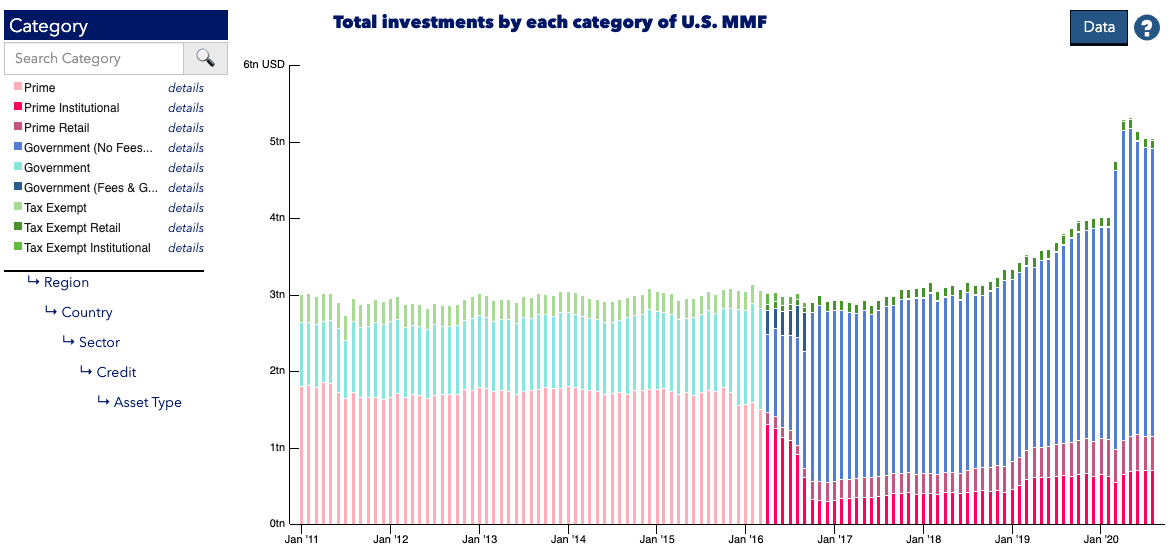
\includegraphics[width=7in]{fig1.png}}
\caption{Total Net Assets of the US Money Market Mutual Fund industry (\$ trillions, monthly)\\
Note: Until October 2016, government and prime money market funds filed Form N-MFP without identify themselves as institutional or retail funds. After that, there was a regulatory change to identify themselves.
\textbf{Source: U.S. SEC Form N-MFP, Office of Financial Research (OFR) Analysis}}
\label{fig:1}
\end{figure}


\paragraph{} In order to limit the risk taking of money market funds, the SEC mandates them to comply with Rule 2a-7 of the Investment Company Act of 1940. Under this rule, money market funds are required to invest only in short-term securities that have the highest credit ratings, and there is an upper bound on the weighted average maturity (WAM) of the portfolio. Funds are also not allowed to invest more than 5\% of their assets in any individual issuer. 

\paragraph{} The funds are divided into retail and institutional on the basis of the type of investors; prime and government funds on the basis of their holdings. They are further divided into taxable and tax-exempt funds. Government funds mainly hold treasuries, government backed agency debt etc. On the other hand, prime funds' holdings comprise of commercial papers, structured securities, bank obligations etc. About two-thirds of the total number of funds are government funds and the rest are prime funds. 


\subsection{Run on Money Market Mutual Funds}

\paragraph{} Money market funds are open-ended mutual funds that invest in low risk short-term securities. As mentioned before, MMMFs main objective is to maintain the principal value of their assets. Hence they adopt a stable Net Asset Value (NAV) of \$1, and if the NAV falls below \$1 the fund is said to have 'broken the buck'. In September 2008, after Lehman Brothers went bankrupt, it's primary financier, the Reserve Primary Fund broke the buck and initiated a run on the MMMFs. This led to a market-wide panic and selloff of other instruments as well. Following this SEC brought in few regulatory reforms (Rule 2a-7), which limits the risk taking of the funds. 

\paragraph{} Similar events happened when there was a growing concern about the health of European banks during the sovereign debt crisis in Europe in 2011. But the magnitude of damage caused by the run on MMMFs and speed with which it happened were milder and more graduate compared to the one that happened in 2008. After several debates between academics and regulators, and recommendations by Financial Stability Oversight Council (FSOC) and the Squam Lake Group (\cite{french2010squam}), the SEC has finally implemented a few reforms in MMMFs on October 14, 2016. As part of these reforms, (i) institutional MMMFs must adopt a floating Net Asset Value (NAV) on their risk-taking behavior, (ii) funds can impose liquidity restrictions, which allows the funds to charge liquidation fee and impose redemption gates after funds' weekly liquid assets fell by 30\%, (iii) retail and institutional share classes must be divided into separate funds, and both prime and government funds have to identify themselves as institutional or retail funds in Form N-MFP.

\paragraph{} Despite these regulatory reforms, MMMF market showed signs of distress in early March 2020. The secondary markets for commercial papers and certificates of deposit became non-existent literally and MMMFs had to rely on their liquidity buffers to fund redemptions. The Federal Reserve stepped in to stabilize and restore liquidity in the short-term lending markets by setting up credit facilities like the Money Market Mutual Fund Liquidity Facility (MMLF) under Section 13(3) of the Federal Reserve Act. This facility administered by the Federal Reserve Bank of Boston provides non-recourse loans (which means the Federal Reserve will take the hit if the security defaults) for banks to purchase short-term securities from MMMFs. The MMLF began its operations on the 23rd of March 2020 and covered investments in commercial papers, asset-backed commercial papers, short-term municipal debt, certificates of deposits and variable-rate demand notes. The MMMF markets were stabilized by the end of March 2020 as seen in the below figure.

\begin{figure}[!htb]
\centerline{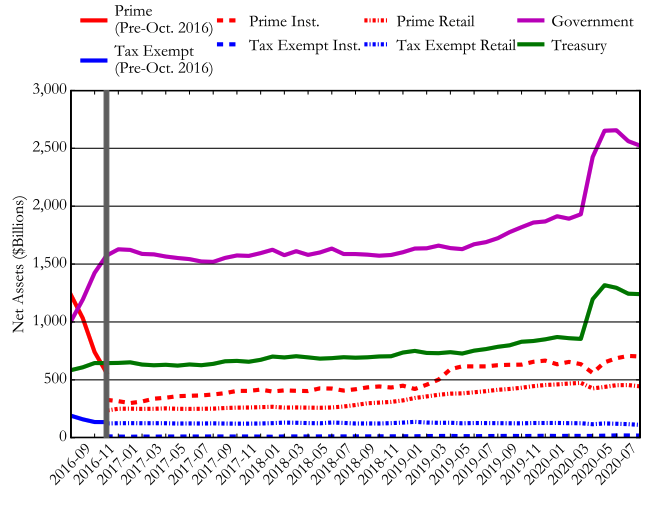
\includegraphics[width=6in]{fig2.png}}
\caption{Net Assets of the US Money Market Funds by category (\$ billions, monthly)\\
\textbf{Source: U.S. SEC Division of Investment Management Analytics Office, Money Market Fund Statistics, Form N-MFP Data, period ending July 2020}}
\label{fig:2}
\end{figure}

The question now is why weren't the regulatory reforms able to stop the run in March 2020? Are the runs on MMMFs inevitable during the crisis? Is government intervention absolutely necessary during the crisis? Further research is needed on how to better predict these runs and stop them from happening.

\section{Literature Review} \label{sec:Lit}

\subsection{Documentation of the events that happened during the financial crisis and the sovereign debt crisis of Europe}

\paragraph{} \cite{strahan2015once} study the risk-taking behavior in money market mutual funds following Lehman Brothers bankruptcy. They show that the money funds that experienced overwhelming outflows met their redemption demands with cash from maturing securities and by liquidating their safest assets. Thus they ended up holding securities which are risky and have longer maturities compared to other funds. Following this, by the end of 2008, these funds reallocated their capital to safer and shorter term assets compared to their portfolio on the eve of Lehman bankruptcy. This could be due to investors’ flight to quality or manager’s career concerns. The authors follow an empirical approach to show this, where they look at how funds’ outflows vary with the proportion of risky assets in their portfolios and gross yields, while using fund controls like fund size, fund family size, expense ratios, weighted average maturity of the portfolio. The authors also show that government guarantees did not result in moral hazard problem in this setting. Which means, the funds backed by capital assistance from the government did not increase their portfolio’s riskiness in long run. 

\paragraph{} \cite{duchin2014safer} do a similar analysis for banks and show that the riskiness in banks’ investments and lending increased after the approval of bailout packages. They say that banks use this money to maintain the capital requirements which gives them an opportunity to take on more risk. Thus there is a serious moral hazard problem in banks. 

\paragraph{} \cite{kacperczyk2013safe} also study the risk-taking behavior of money market mutual funds during the financial crisis. According to them, money market funds act as intermediaries between issuers of debt and the investors. If money market funds have strong incentives to take on risk, this layer of financial intermediation destabilizes the wider economy by reducing market discipline of the corporations and financial institutions, thus making a run on them inevitable. The authors show that the money market funds experienced an increase in risk-taking opportunities from mid 2007. The investors were more responsive to higher fund yields as they poured in more money into the funds. In their empirical analysis, the authors show that one standard deviation increase in fund yields led to 43\% increase in the fund asset size. They also show that the fund sponsors who had multiple money market fund businesses took on more risk. A one standard deviation increase in the size of prime institutional money market fund assets led to the increase of: 3.7\% of risky asset holdings, 2.3 days of weighted average maturity of the portfolio, 3\% of fund yields. They further show that the sponsors who had less money market fund businesses or businesses other than money funds avoided taking risk and hence ended up having less outflows during the run of these funds. These sponsors were more likely to provide capital assistance in case of a run on the MMMFs, and are highly likely to exit the money fund business within 2 years or change their name following the crisis.

\paragraph{} \cite{chernenko2014frictions} reinforce the results of \cite{kacperczyk2013safe,strahan2015once}. They show that risky MMMFs which have greater exposures to the European banks experienced larger outflows during the summer of 2011, when sovereign risk concerns mounted. The authors also show that the funds’ exposure to European banks decreased the access to financing for the non-European issuers (even creditworthy firms) due to frictions in the credit market. The authors use security-level holdings data for their empirical analysis, which eliminates identification problems as issuers’ financing could also come through bank-lending. In their empirical analysis, the authors look at the relation between change in the share of issuer in the funds’ portfolio with exposure to European banks and strength of issuer-fund relationships. In contrast with earlier literature, they show that relationships between issuers and MMMFs matter, as funds in distress cutdown lending to issuers with whom they have weaker relationship. 

\paragraph{} \cite{schmidt2016runs} develop a static coordination game with strategic complementarities (i.e., concerns about negative externalities from the redemptions of other investors) and asymmetric information to predict the relationship between sophistication level of the investors and outflows of the fund, and test their theory empirically. Sophisticated investors are well informed about the fundamentals of the fund holdings, and possess both public and private information. The authors focus on pooling equilibria (perfect Bayesian equilibria) wherein informed (sophisticated) investors have an incentive to withdraw funds if the private signal is below a certain value. This value is very low for the informed investors compared to the uninformed ones, hence the probability that the informed investors attacks (withdraws) is high. In their empiricial analysis, the authors show that outflows of sophisticated investors is greater than unsophisticated investors when there is negative fundamental shock in a particular fund. Following the shock, funds with higher concentration of sophisticated investors have a larger difference between sophisticated and unsophisticated investor outflows. The authors use expense ratios to distinguish between share classes of sophisticated and unsophisticated investors. Finally, they show that the sponsors with businesses other than MMMF avoid taking risk in order to safeguard their other businesses. 

\paragraph{} \cite{gallagher2020investor} study how investors' (particularly sophisticated investors) acquisition of more information about MMMFs' risk exposures affect their redemptions from the fund and portfolio rebalancing decisions of the manager.
They say investors rationally choose not to waste their resources on information acquisition during regular times, as the incentives are very low. But when liquidity dries up suddenly and rapidly, investors' concerns escalate overnight. This generates incentives to accumulate more information about the credit quality of MMMFs' assets, strategic complementarities etc. (see \cite{schmidt2016runs}). In this information-sensitive environment, investors' perception of the MMMFs' risk exposures change completely from before. This leads to MMMF portfolio managers rebalancing and avoiding exposures to information-sensitive securities in their holdings, in order to alleviate investor concerns, after experiencing overwhelming redemptions (consistent with \cite{strahan2015once}). The authors study this mechanism during the 2011-12 sovereign debt crisis in Europe. They compare funds with similar ex-ante risk levels and show empirically that managers who serve sophisticated investors (who acquire the most information) rebalance their holdings away from the Euro zone credit risk exposure more, while increasing exposures to other regions. The credit risk measure used here is 'expected loss to maturity' of the fund, which is estimated from the default probabilities that match securities' time to maturity.


\subsection{Evaluation of the proposed regulatory reforms in MMMFs (ex-ante)}

\paragraph{} \cite{hanson2015evaluation} evaluate certain regulatory reforms in MMMFs proposed by the U.S. SEC before they were implemented. There is still heated debate in terms of the regulatory reforms between both schools of thought--where the first school argues that the shadow banking system is very similar to traditional banks hence should be regulated like them, and the second school argues that they should be subjected fully to market forces and should not be bought under the bank regulatory purview. Reforms are supposed to cut down ex-ante incentives for MMMFs to take on more risk and improve the ex-post chances of resilience of them to market-wide runs. The authors show that the subordinated capital buffer could be effective in achieving these goals. They say the capital buffer should be 3\%-4\% of the fund assets for a well-diversified portfolio, and higher for concentrated portfolios. The Minimum Balance at Risk (MBR) proposal, according to which, the investors cannot redeem 3\% of their assets for 30 days after redeeming the rest, is essentially like a capital buffer. Both capital buffer and MBR take the first loss in case the fund breaks the buck. In contrast with \cite{schmidt2016runs} results, \cite{hanson2015evaluation} say that the floating NAV proposal will not be effective in eliminating a run during the crisis as it may not change investor's risk preferences as long as they can redeem their shares on demand; the NAV value does not change much as the assets held by MMMFs are illiquid; investors still want to sell their shares at discount in the case of a run. They also say that the increased transparency by Rule 2a-7 has not minimized the incentives of investors to chase high yields; news that one fund imposed redemption restrictions could start a run on other funds as investors want to redeem their fund imposes restrictions. Finally, the authors propose that the reforms should also aim to reduce the impact of MMMF runs on the wider economy, and financial institutions' incentives to bank excessively upon the unstable and short-term financing from MMMFs.  

\paragraph{} \cite{adrian2016shadow} study the regulatory reforms in MMMFs proposed by the Financial Stability Oversight Council (FSOC) and the Squam Lake Group (SLG). Consistent with \cite{hanson2015evaluation}, the authors say that the investors of MMMFs consider them as demand deposits because of their stable \$1 NAV rule. However if they abandon it and adopt floating NAVs, it need not necessarily be beneficial to MMMFs. Floating NAVs would not eliminate the incentives for investors to run, and quote some instances in the Europe where the run on MMMFs has happened despite adopting floating NAVs. The authors say the ex-ante and ex-post buffers will help prevent the runs as they take the first hit in case of a system-wide panic. The authors also evaluate SLG's proposal for MMMFs to adopt two tranches/share classes, where the senior tranche would be fixed \$1 NAV and is provided a liquidity buffer, whereas the junior tranche will adopt a floating NAV. They say the two tranche proposal will not protect the funds from runs in all states of the world.  

\subsection{Impact of the bank regulatory reforms on shadow banking sector}
\paragraph{} On the policy front in banks, \cite{diamond1983bank} develop a theoretical model to show that there exists a demand deposit contract issued by banks that would prevent runs on the banks and also shares the risk optimally among the depositors by transforming illiquid assets to liquid, when deposit insurance by the government is available. Banks are able to convert illiquid securities by offering different liabilities with smoother returns.  The authors show that banks' demand deposit contracts providing such capabilities have multiple equilibria. One of which is a desirable equilibrium wherein there is efficient risk sharing among the depositors and the other is an undesired equilibrium wherein all the depositors panic and cause a bank run. Bank runs cause serious damage to the broader economy as the probability of failing of even healthy banks increase, and they act by recalling the loans thus causing interruptions in production. This is an undesirable outcome, hence contracts are required to eliminate such inefficiencies in the system.

\paragraph{} \cite{plantin2015shadow} talks about how regulations on the traditional banks induce shadow banking activity. As mentioned in section-\ref{sec:Intro}, MMMFs and other shadow banks exist because of the regulatory arbitrage between these institutions and the regular banks. The author develops a theoretical model to study the most efficient bank regulation on their capital requirements in the presence of such an arbitrage. He shows that tightening capital requirements is inefficient because it gets more costly for banks to bear adverse selection risks, and hence lead to the banks offloading more risk than necessary into the shadow banking facilities in order to bypass the bank capital requirements. This will lead to banks ending up being exposed to higher aggregate risk of money-like liabilities of the shadow banking system.  

\paragraph{} \cite{xiao2020monetary} explores a new explanation for the diminished impact of monetary policy. He therefore looks at the impact on the shadow banking activity through monetary transmission, and shows how it negatively impacts traditional bank deposits. He develops a theoretical model of bank competition to show that in contrast with traditional banks, shadow bank deposits expand during the cycles of monetary tightening. This is because shadow banks pass on most of the yields to their depositors who are highly sensitive to yields, thus attracting more deposits. He also shows that this leads to reduction of about one-thirds of the commercial bank deposits, thereby dampening the monetary transmission. The author explains this by introducing heterogeneous preferences of clientele and product differentiation for deposits between traditional and shadow banks in his model. He finally shows that its not the differences in capital requirements or default risks that differentiate shadow banks from regular banks, but the different depositor clientele.

\subsection{Effect of the regulatory reforms in MMMFs (ex-post analysis)}

\paragraph{} \cite{li2020runs} study the impact of regulatory reforms in MMMFs implemented in late 2016. They specifically study the liquidation restriction, which allows the funds to charge liquidation fee and impose redemption gates after certain withdrawal limit (30\% of the funds assets in a week). They show that these reforms have actually exacerbated the run on prime funds during the Covid-19 crisis. This was because of the preemptive run caused when the funds' liquidity buffer fell by a certain threshold, as the investors felt that funds might impose these restrictions. The authors also compare the magnitude of damage caused by runs on MMMFs in 2020 with those happened during 2008 and 2011. They find both 2020 and 2008 runs are equivalent in terms of speed and intensity; outflows were highly sensitive to funds' liquidity in 2020 compared to 2008. In 2020 crisis, one standard deviation (6.4\%) decrease in weekly liquid assets led to 0.9\% increase in outflows compared to regular times. This suggests that liquidity restriction reform has caused more damage than good. The authors also study the effect of Money Market Mutual Fund Liquidity Facility (MMLF) on the condition of prime funds. They use micro-level data from MMLF to show how MMLF-eligible funds are stabilized in comparison with MMLF-ineligible funds which invest in the same commercial papers and certificates of deposit. Finally, using holdings data from Form N-MFP they show that funds holding more MMLF-eligible securities recover quicker in terms of the inflows following the setup of MMLF.

\paragraph{} \cite{baghai2020liability} study how the regulatory reforms affected the funds' and depositors' investing behavior and had unintended consequences in the economy. They show that following the reforms, inflows into prime funds became more responsive to their performance. Moreover sophisticated investors started accumulating more information to extract more returns (as retail share classes were separated to start a new fund), making it difficult for prime funds to survive (consistent with \cite{gallagher2020investor}). The affected funds therefore responded by taking on more risk and cutting down overall funding provided to corporations (even creditworthy firms). The authors show the increase in risk-taking behavior in institutional funds from their increase of portfolio spreads compared to those of retail funds, and increase in the proportion of their investments in risky securities. The authors show that the cut down of access to funding by MMMFs is not due to decrease in demand by corporations, and use security-level data to show this cut down is even more pronounced for safer borrowers. They also say that extending more funding to riskier firms led to an increase in volatility in money markets, which ended up causing a market-wide panic during the Covid-19 crisis.

\clearpage
% Bibliography.

\begin{doublespacing}   % Double-space the bibliography
\bibliographystyle{jf}
\bibliography{bibliography}
\end{doublespacing}

\end{document}

